%% ------- ROZDZIAŁ 4 ------- %%

\chapter{Testy aplikacji}

\section{Cel przeprowadzonych analiz}

Wykorzystując napisaną na potrzeby niniejszej pracy aplikację przeprowadzono testy, które zmierzają do porównania wybranych modeli regresji dostępnych w pakiecte \textit{Scikit-learn}.\\

Testy przeprowadzone zostały na dwóch zbiorach danych: cen giełdowych firmy Microsoft w zakresie od 2017-01-01 do 2017-10-30, oraz cen giełdowych firmy Intel w zakresie od 2017-01-01 do 2017-04-30.
W dlaszej części zbiory te będą nazywane odpowiednio: zbiór szeroki i zbiór wąski.
Dane wykorzystane do testów były cenami otwarcia.\\

Każdy przeprowadzony test uwzględnia wyliczenie dwóch wartości: średniego błędu kwadratowego oraz wyniku predycji.\\

Średni błąd kwadratowy liczony jest poprzez wykorzystanie funknji \textit{sklearn.metrics.mean\_squared\_error} z pakietu \textit{Scikit-learn}, a jego wartość w wypadku predykcji idealnej wynosi zero.
Liczony jest na podstawie wartości predykcji dla danych testowych.
Wynik predykcji jest natomiast liczony poprzez wywołanie metody \textit{score()} obieku danego modelu regresji, a jego wartość zmierza do osiągnięcia 1.0 w przypadku idealnym.
Liczony jest na podstawie wyników predykcji zarówno dla zbioru uczącego jak i testowego.\\

Przeprowadzono osobne testy dla każdej z trzech wartości procentowych ilości danych uczących w stosunku do ilości danych testowych: 20\%, 50\% oraz 80\%.\\

Wybrane modele regresji to:
\begin{itemize}
 \item Regresja Liniowa
 \item Regresja Grzbietowa (KRR)
 \item Regresja Wektorów Nośnych (SVR)
 \item Regresja Procesu Gaussa (GPR)
\end{itemize}

Reasumując, dla każdej z metod regresji wykonano sześć testów.\\

Celem testów jest porównanie modeli regresji dostępnych w pakiecie \textit{Scikit-learn} i wyciągnięcie wniosków dotyczących:
\begin{itemize}
 \item dokładności predykcji modeli w zależności od ilości danych uczących oraz całkowitej ilości danych
 \item zdolności modeli do reprezentacji trendu
 \item wpływu zmiany ilości danych uczących na dopasowanie modeli
 \item wpływu całkowitej ilości danych na dopasowanie modeli
\end{itemize}



\section{Testy zbioru danych: Microsoft}

\subsection{Informacje ogólne}
Zakres danych użytych do testów wynosi 209 próbek, w przedziale dat od 2017-01-01 do 2017-10-30 z krokiem wynoszącym jeden dzień.\\

\begin{figure}[h!]
\centering
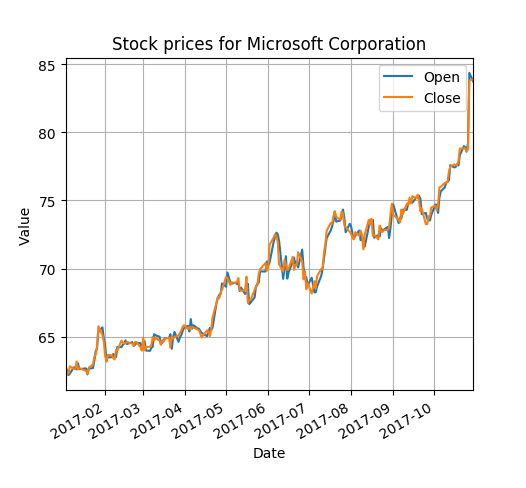
\includegraphics[width=150mm]{pictures/plots/microsoft_oc_price.png}
\caption{Wykres cen otwarcia i zamknięcia firmy Microsoft}
\label{fig:microsoft_oc_price}
\end{figure}

Na rysunku \ref{fig:microsoft_oc_price} przedstawiono wykres zmian cen otwarcia i zamknięcia dla podanego zakresu dat.\\ 

Ilość próbek danych uczących i testowych wynosi odpowiednio:
\begin{itemize}
 \item 41/168 dla wartości 20\% danych uczących
 \item 104/105 dla wartości 50\% danych uczących
 \item 167/42 dla wartości 80\% danych uczących
\end{itemize}
Na przedstawionych wykresach zaznaczona została linia podziału danych uczących i testowych i jest ona reprezentowana przez czerwoną pionową prostą.

\subsection{Regresja liniowa}
Wykres regresji liniowej dla podanego zbioru danych, przy proporcji 20\% danych uczących przedstawiony jest na rysunku \ref{fig:microsoft_linear_20}.\\

\begin{figure}[h!]
\centering
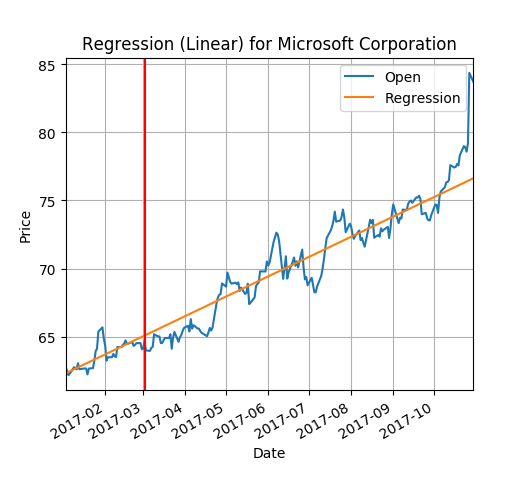
\includegraphics[width=150mm]{pictures/plots/microsoft_linear_20.png}
\caption{Wykres regresji liniowej dla 20\% danych uczących, Microsoft}
\label{fig:microsoft_linear_20}
\end{figure}

Widoczny jest tu trend wzrostowy, który określony na podstawie danych uczących, kontunuowany jest także dla danych testowych.
Należy jednak zauważyć, że podany zbiór danych nie zawiera gwałtownych wzrostów i spadków cen w szczególności w części testowej, dzięki czemu regresja z powodzeniem przewiduje jego kontynuację.\\

Na rysunku \ref{fig:microsoft_linear_50} przedstawiono wykres regresji liniowej dla 50\% proporcji danych uczących.
\begin{figure}[h!]
\centering
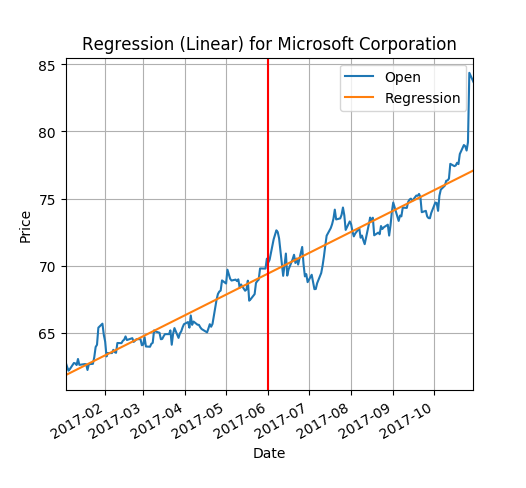
\includegraphics[width=150mm]{pictures/plots/microsoft_linear_50.png}
\caption{Wykres regresji liniowej dla 50\% danych uczących, Microsoft}
\label{fig:microsoft_linear_50}
\end{figure}

Porównując wykresy \ref{fig:microsoft_linear_20} oraz \ref{fig:microsoft_linear_50} zauważalne jest niewielkie przesunięcie prostej regresji w kierunku niższej ceny, 
choć mimo tego można stwierdzić, że dla danego zbioru danych zwiększenie wartości podziału danych na testowe i uczące nie miało wpływu na wynik.

Rysunek \ref{fig:microsoft_linear_80} przedstawia wykres regresji liniowej dla 80\% proporcji danych uczących.\\

\begin{figure}[h!]
\centering
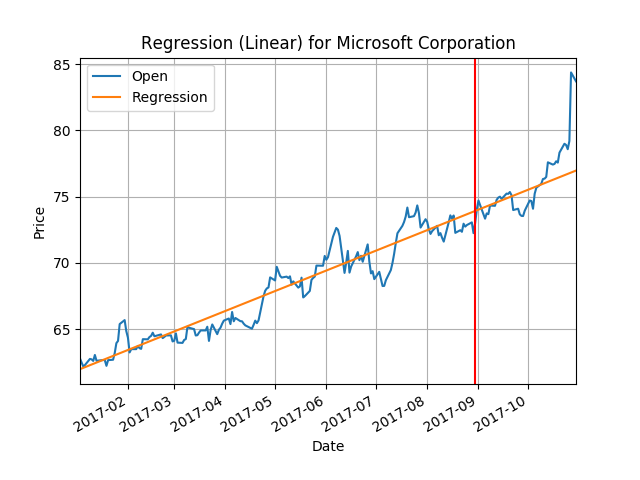
\includegraphics[width=150mm]{pictures/plots/microsoft_linear_80.png}
\caption{Wykres regresji liniowej dla 80\% danych uczących, Microsoft}
\label{fig:microsoft_linear_80}
\end{figure}

W porównaniu do regresji liniowej przeprowadzonej dla 20\% i 50\% danych uczących, wyniki regresji przeprowadzonej dla 80\% danych uczących nie różnią się wiele od pozostałych.
Zauważalne jest jedynie delikatne przesunięcie prostej regresji w kierunku cen niższych, co może być spowodowane przez zmiany kierunku mniejszych trendów obecnych na wykresie.

\subsection{Regresja Grzbietowa}

Rysunki \ref{fig:microsoft_krr_20}, \ref{fig:microsoft_krr_50} i \ref{fig:microsoft_krr_80} przedstawiają wyniki regresji grzbietowej dla 20\%, 50\% i 80\% użytych danych uczących.\\

\begin{figure}[h!]
\centering
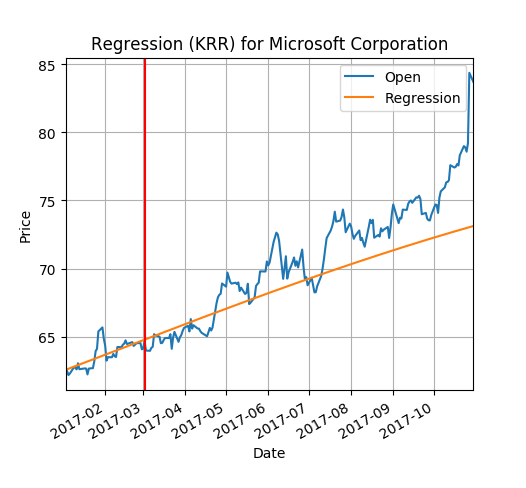
\includegraphics[width=150mm]{pictures/plots/microsoft_krr_20.png}
\caption{Wykres regresji grzbietowej dla 20\% danych uczących, Microsoft}
\label{fig:microsoft_krr_20}
\end{figure}

Krzywa regresji widoczna na powyższym rysunku nie posiada dużych odchyleń, co upodabnia ją do prostej regresji liniowej.
Odchylenie jest zauważalne dopiero przy końcowej części danych testowych. Fakt ten może być spowodowany zbyt małą liczbą danych uczących użytych do przeprowadzenia analizy.\\

\begin{figure}[h!]
\centering
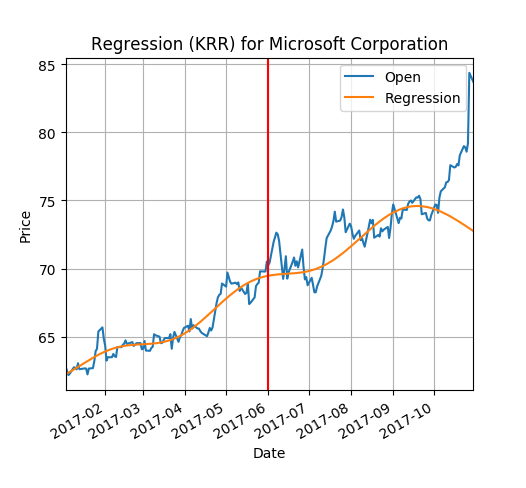
\includegraphics[width=150mm]{pictures/plots/microsoft_krr_50.png}
\caption{Wykres regresji grzbietowej dla 50\% danych uczących, Microsoft}
\label{fig:microsoft_krr_50}
\end{figure}

W porównaniu do rysunku \ref{fig:microsoft_krr_20}, powyższy wykres przedstawia wynik bardziej dokładny i dopasowany.
Zaznaczony jest wyraźny trend wzrostowy z dopasowanymi krzywiznami, które trafnie pokrywają dużą część danych testowych.\\

\begin{figure}[h!]
\centering
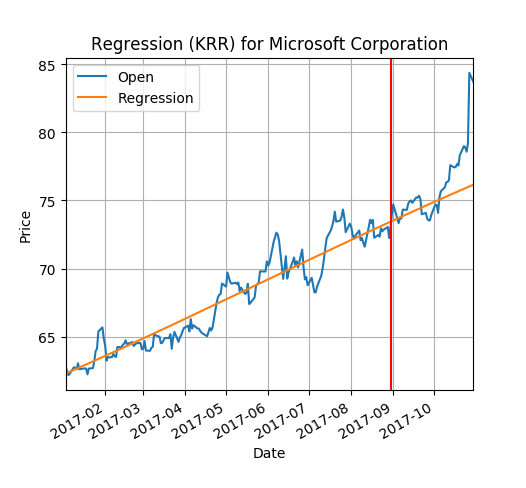
\includegraphics[width=150mm]{pictures/plots/microsoft_krr_80.png}
\caption{Wykres regresji grzbietowej dla 80\% danych uczących, Microsoft}
\label{fig:microsoft_krr_80}
\end{figure}

Wykres przedstawiający wyniki regresji grzbietowej dla największej ilości zastosowanych danych testowych przedstawia krzywą regresji zbliżoną kształtem do prostej.
Może to być spowodowane zastosowaniem zbyt dużej ilości danych uczących, które znajdują się w wyraźnym wzrostowym trendzie o niewielkich odchyleniach.\\

\subsection{Regresja Wektorów Nośnych}

Rysunki \ref{fig:microsoft_svr_20}, \ref{fig:microsoft_svr_50} i \ref{fig:microsoft_svr_80} przedstawiają wykresy wyników regresji wektorów nośnych dla wskazanego zbioru danych, 
o podziale danych uczących względem danych testowych odpowiednio: 20\%, 50\% i 80\%.\\

\begin{figure}[h!]
\centering
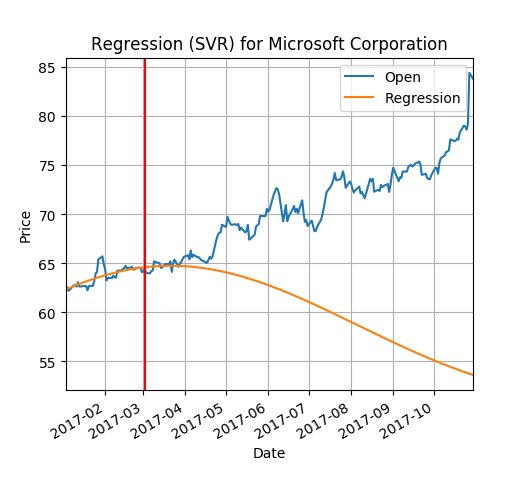
\includegraphics[width=150mm]{pictures/plots/microsoft_svr_20.png}
\caption{Wykres regresji wektorów nośnych dla 20\% danych uczących, Microsoft}
\label{fig:microsoft_svr_20}
\end{figure}

W powyższym przypadku regresja wektorów nośnych wykazuje bardzo niewielkie zdolności predykcyjne, a także niewielkie dopasowanie modelu.
Krzywa regresji po osiągnięciu granicy danych uczących, znacząco odchyla się w kierunku dolnym, coraz bardziej zwiększając błąd predykcji.\\

\begin{figure}[h!]
\centering
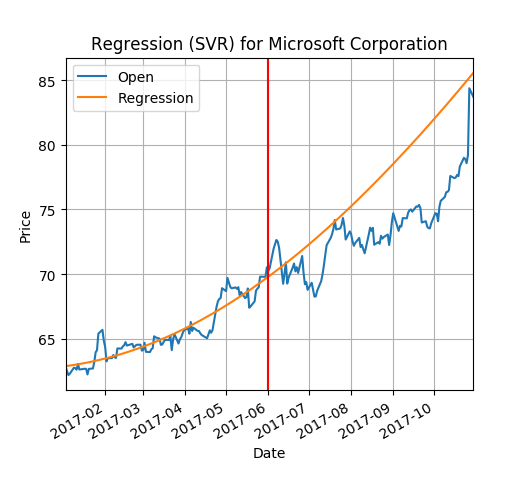
\includegraphics[width=150mm]{pictures/plots/microsoft_svr_50.png}
\caption{Wykres regresji wektorów nośnych dla 50\% danych uczących, Microsoft}
\label{fig:microsoft_svr_50}
\end{figure}

W odróżnieniu od krzywej regresji na rysunku \ref{fig:microsoft_svr_20}, w powyższym przypadku krzywa ta poprawnie przewiduje trend wzrostowy.
Jednakże odchylenie krzywej w stronę górną jest tak silne, że wraz ze wzrostem wartości na osi X wykresu, spada dopasowanie danych.\\

\begin{figure}[h!]
\centering
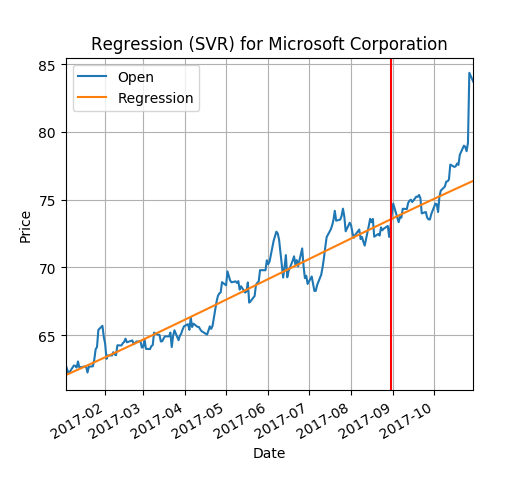
\includegraphics[width=150mm]{pictures/plots/microsoft_svr_80.png}
\caption{Wykres regresji wektorów nośnych dla 80\% danych uczących, Microsoft}
\label{fig:microsoft_svr_80}
\end{figure}

Na wykresie \ref{fig:microsoft_svr_80} można zaobserwować krzywą regresji wektorów nośnych, która przyjmuje postać prostej.
Zachowanie to jest zbieżne z zaobserwowanym na wykresach regresji grzbietowej, co może prowadzić do umocnienia wniosku o użytej zbyt dużej ilości danych uczących przy fakcie, iż dane te reprezentują silny trend wzrostowy.\\

\subsection{Regresja Procesu Gaussa}

Rysunki \ref{fig:microsoft_gpr_20}, \ref{fig:microsoft_gpr_50}, \ref{fig:microsoft_gpr_80} przedstawiają wykresy wyników analiz regresji procesu Gaussa dla odpowiednio: 20\%, 50\% i 80\% zastosowanych danych uczących.\\

\begin{figure}[h!]
\centering
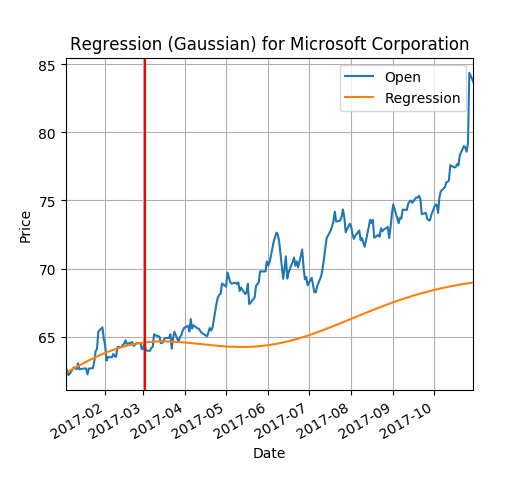
\includegraphics[width=150mm]{pictures/plots/microsoft_gpr_20.png}
\caption{Wykres regresji procesu Gaussa dla 20\% danych uczących, Microsoft}
\label{fig:microsoft_gpr_20}
\end{figure}

Na powyższym wykresie możemy zaobserwować zachowanie się krzywej regresji, któ©e jest bardzo podobne do tej z rysunku \ref{fig:microsoft_svr_20}.
Spowodowane to może być zbyt małą ilością użytych danych uczących, które charakteryzują się niewielką zmiennością.\\

\begin{figure}[h!]
\centering
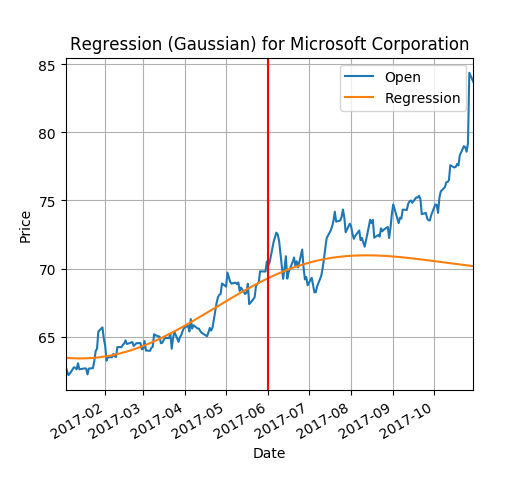
\includegraphics[width=150mm]{pictures/plots/microsoft_gpr_50.png}
\caption{Wykres regresji procesu Gaussa dla 50\% danych uczących, Microsoft}
\label{fig:microsoft_gpr_50}
\end{figure}

Wykres na rysunku \ref{fig:microsoft_gpr_50} powtarza tendencję z wykresu na rysunku \ref{fig:microsoft_gpr_20}.
Trend wzrostowy jest poprawnie predykcjonowany jedynie dla początkowych wartości danych testowych, a następnie występuje odchylenie krzywej regresji w dół.\\

\begin{figure}[h!]
\centering
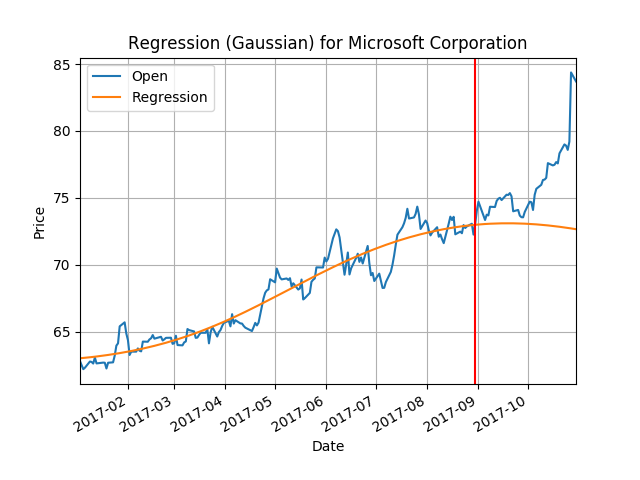
\includegraphics[width=150mm]{pictures/plots/microsoft_gpr_80.png}
\caption{Wykres regresji procesu Gaussa dla 80\% danych uczących, Microsoft}
\label{fig:microsoft_gpr_80}
\end{figure}

Krzywa regresji na powyższym wykresie w odróżnieniu od pozostałych nieliniowych metod regresji, nie wykazuje tendencji do zbliżania się kształtem do prostej.
Jednak predykcja dla zbioru testowego, oraz trend jaki wskazuje krzywa, gorzej odzwierciedlają rzeczywiste dane.\\

\subsection{Podsumowanie}

Podczas dokonanych analiz zebrano dane odnośnie wartości średniego błędu kwadratowego każdej z nich, a także wyniku predykcji. Przedstawiono je na wykresach znajdujących się na rysunkach \ref{fig:microsoft_mean_square} i \ref{fig:microsoft_score}.\\

\begin{figure}[h!]
\centering
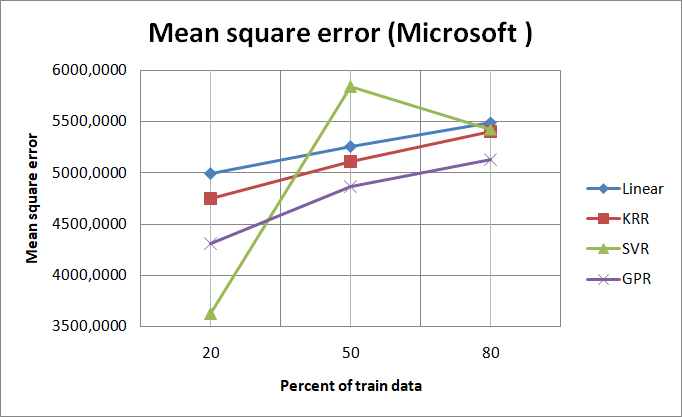
\includegraphics[width=150mm]{pictures/plots/microsoft_mean_square.png}
\caption{Wykres zmian wartości średniego błędu kwadratowego, Microsoft}
\label{fig:microsoft_mean_square}
\end{figure}

\begin{figure}[h!]
\centering
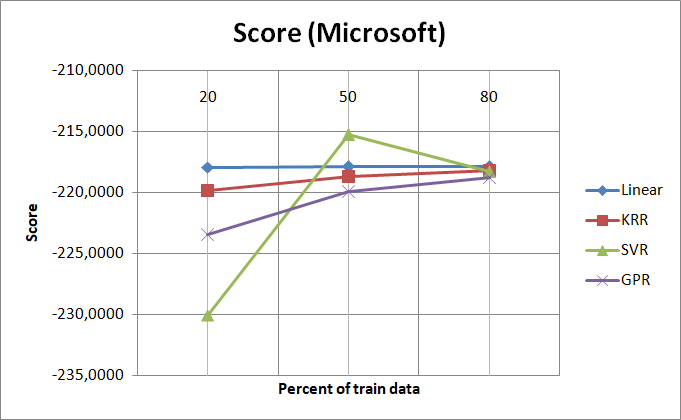
\includegraphics[width=150mm]{pictures/plots/microsoft_score.png}
\caption{Wykres zmian wartości wyników dopasowania modelu, Microsoft}
\label{fig:microsoft_score}
\end{figure}

Z powyższych wykresów wynika, iż średni błąd kwadratowy rośnie wraz ze wzrostem ilości danych uczących zastosowanych w analizie.
Wynik predycji natomiast odznacza się niewielkim wzrostem wraz ze zwiększaną ilością danych uczących.\\

Dla 20\% zastosowanych danych uczących najmniejszy błąd osiągnęła regresja wektorów nośnych, zaś największy - liniowa.
W przypadku wyniku predykcji jest natomiast odwrotnie: najlepszą wartość osiągnęła regresja liniowa,  a najgorszą regresja wektorów nośnych.\\

Dla 50\% zastosowanych danych uczących najmniejszym błędem kwadratowym charakteryzuje się regresja procesu Gaussa, a najwyższym regresja wektorów nośnych.
Powtórzona zostaje zależność zidentyfikowana w przypadku 20\% danych uczących: wynik predykcji oceniany najlepiej należy do regresji wektorów nośnych, natomiast najgorzej do regrtesji procesu Gaussa\\

W przypadku 80\% zastosowanych danych testowych regresja procesu Gaussa osiągnęła najniższy wynik średniego błędu kwadratowego. Pozostałe modele regresji charakteryzują się zbliżonym wynikiem.
Wynik predykcji dla każdego z modeli jest w tym przypadku bardzo zbliżony.\\

Na podstawie zgromadzonych wykresów, a także powyższych danych, można określić następujące wnioski:
\begin{itemize}
 \item trafne określenie trendu dla danych testowych zaobserwowano w przypadkach regresji liniowej, wektorów nośnych (80\% danych uczących) oraz grzbietowej (20\% i 80\% danych uczących)
 \item krzywe regresji, które nie identyfikowały poprawnie trendu dla danych testowych należą do regresji wektorów nośnych (20\% danych testowych) oraz procesu Gaussa
 \item w przypadku regresji grzbietowej (50\% danych uczących), zaobserwowano dobre dopasowanie i potwierdzenie trendu dla około 80\% danych testowych, po czym następowała zmiana nachylenia krzywej
\end{itemize}


\section{Testy zbioru danych: Intel}

\subsection{Informacje ogólne}
Zakres danych użytych do testów wynosi 81 próbek, w przedziale dat od 2017-01-01 do 2017-14-30 z krokiem wynoszącym jeden dzień.\\
Zakres ten charakteryzuje się mniejszą ilością danych o większej zmienności, niż zakres poprzedni.

\begin{figure}[h!]
\centering
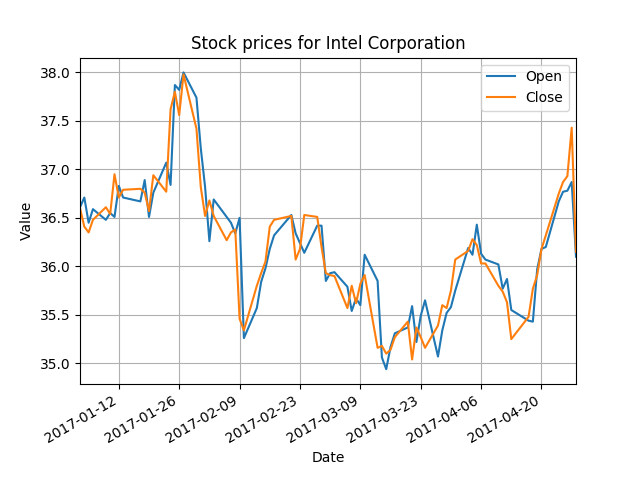
\includegraphics[width=150mm]{pictures/plots/intel_oc_price.png}
\caption{Wykres cen otwarcia i zamknięcia firmy Intel}
\label{fig:intel_oc_price}
\end{figure}

Na rysunku \ref{fig:intel_oc_price} przedstawiono wykres zmian cen otwarcia i zamknięcia dla podanego zakresu dat.\\ 

Ilość próbek danych uczących i testowych wynosi odpowiednio:
\begin{itemize}
 \item 16/65 dla wartości 20\% danych uczących
 \item 40/41 dla wartości 50\% danych uczących
 \item 64/17 dla wartości 80\% danych uczących
\end{itemize}

\subsection{Regresja liniowa}

Na wykresach \ref{fig:intel_linear_20}, \ref{fig:intel_linear_50} oraz \ref{fig:intel_linear_80} przedstawiono wyniko regresji liniowej o udziale danych uczących odpowiednio: 20\%, 50\% i 80\%.\\

\begin{figure}[h!]
\centering
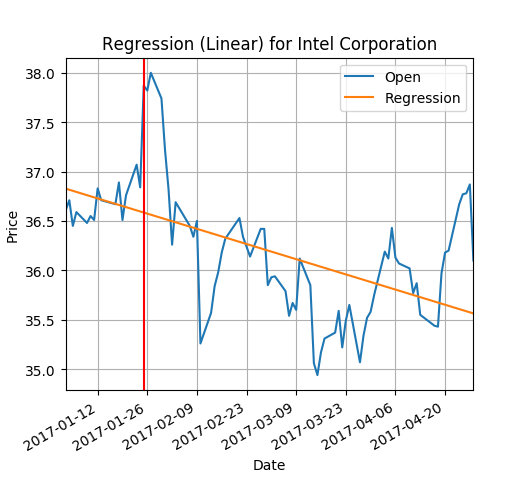
\includegraphics[width=150mm]{pictures/plots/intel_linear_20.png}
\caption{Wykres regresji liniowej dla 20\% danych uczących, Intel}
\label{fig:intel_linear_20}
\end{figure}

Z powyższego wykresu wynika, iż poprzez predykcję poprawnie zidentyfikowano trend spadkowy.\\

\begin{figure}[h!]
\centering
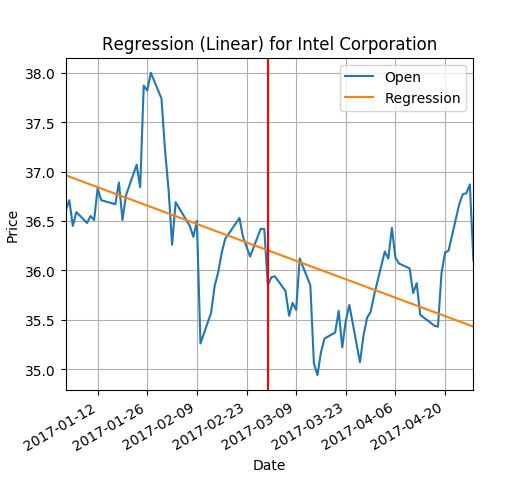
\includegraphics[width=150mm]{pictures/plots/intel_linear_50.png}
\caption{Wykres regresji liniowej dla 50\% danych uczących, Intel}
\label{fig:intel_linear_50}
\end{figure}

W porównaniu do wykresu na rysunku \ref{fig:intel_linear_50}, na powyższym wykresie zaobserwować można prostą regresji identyfikującą trend spadkowy, lecz o mniejszym nachyleniu niż poprzednio.
Może być to spowodowane lepszym dopasowaniem modelu, lub też zwiekszoną liczbą danych uczących.\\

\begin{figure}[h!]
\centering
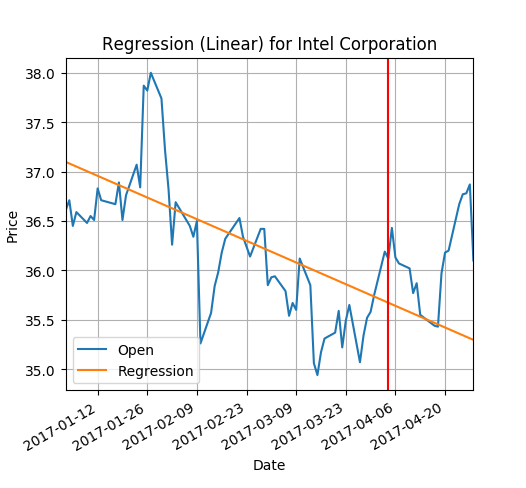
\includegraphics[width=150mm]{pictures/plots/intel_linear_80.png}
\caption{Wykres regresji liniowej dla 80\% danych uczących, Intel}
\label{fig:intel_linear_80}
\end{figure}

Porównując wszystkie trzy powyższe analizy regresji liniowej, można zaobserwować zależność spadku nachylenia prostej regresji od ilości zastosowanych danych uczących.

\subsection{Regresja Grzbietowa}

Na rysunkach \ref{fig:intel_krr_20}, \ref{fig:intel_krr_50} i \ref{fig:intel_krr_80} przedstawiono wyniko analizy regresji grzbietowej, przy zastosowaniu 20\%, 50\% i 80\% danych uczących.\\

\begin{figure}[h!]
\centering
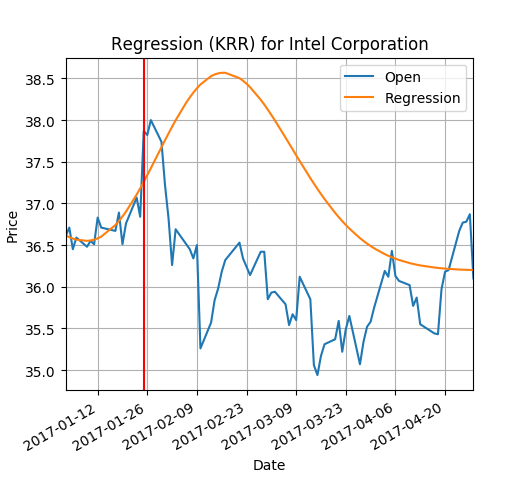
\includegraphics[width=150mm]{pictures/plots/intel_krr_20.png}
\caption{Wykres regresji grzbietowej dla 20\% danych uczących, Intel}
\label{fig:intel_krr_20}
\end{figure}

Powyższy wykres wykazuje błędną predykcję i rozpoznanie trendu, które mogą być skutkiem zbyt małej ilości danych uczących.
Poza tym, dane zakres danych testowych obejmuje jedynie mniejszy trend wzrostowy, przez co utrudniona lub niemożliwa jest identyfikacja szerszego trendu spadkowego.\\

\begin{figure}[h!]
\centering
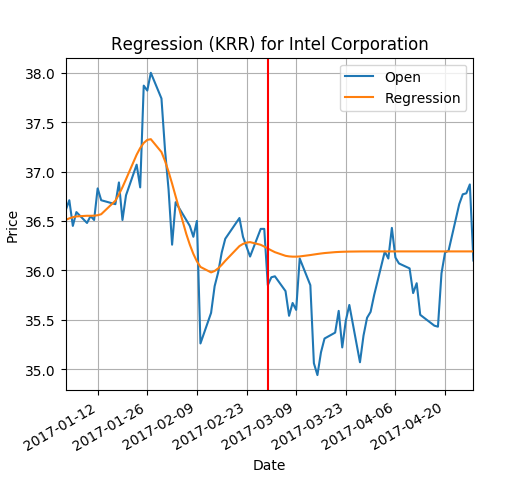
\includegraphics[width=150mm]{pictures/plots/intel_krr_50.png}
\caption{Wykres regresji grzbietowej dla 50\% danych uczących, Intel}
\label{fig:intel_krr_50}
\end{figure}

Wykres \ref{fig:intel_krr_50} przedstawia krzywą regresji, która charakteryzuje się dobrym dopasowaniem w części danych uczących, lecz w części danych testowych staje się ona niemal linią prostą.
Może być to ponownie spowodowane nietrafnie dobranym zakresem danych uczących, ponieważ można w nim zaobserwować zarówno duży wzrost i duży spadek, co w połączeniu z małą ilością próbek danych może czynić zbiór niereprezentacyjnym.\\

\begin{figure}[h!]
\centering
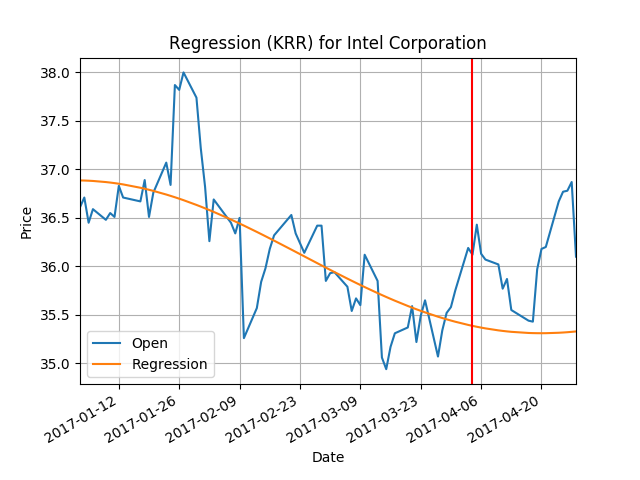
\includegraphics[width=150mm]{pictures/plots/intel_krr_80.png}
\caption{Wykres regresji grzbietowej dla 80\% danych uczących, Intel}
\label{fig:intel_krr_80}
\end{figure}

Spośród trzech przedstawionych analiz regresji grzbietowej, wykres na rysunku \ref{fig:intel_krr_80} zdecydowanie przedstawia krzywą regresji najlepiej przedstawiającą trend.
Należy jednak zauważyć, iż fragment przedstawiający dane testowe jest relatywnie niewielki, a przeidywane wartości nie pokrywają się w żdnym punkcie z wartościami testowymi.\\

\subsection{Regresja Wektorów Nośnych}

Rysunki \ref{fig:intel_svr_20}, \ref{fig:intel_svr_50} i \ref{fig:intel_svr_80} przedstawiają wykresy analizy regresji wektorów nośnych dla proporcji danych uczących wynoszących odpowiednio: 20\%, 50\% i 80\%.\\

\begin{figure}[h!]
\centering
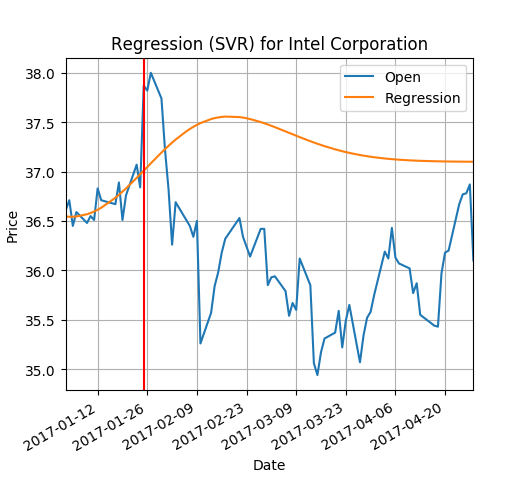
\includegraphics[width=150mm]{pictures/plots/intel_svr_20.png}
\caption{Wykres regresji wektorów nośnych dla 20\% danych uczących, Intel}
\label{fig:intel_svr_20}
\end{figure}

Powyższy wykres przedstawia podobną zależność, co wykres analizy regresji grzbietowej dla tych samych ilości danych uczących.
Podtrzymany zostaje więc wniosek, iż niepoprawna identyfikacja trendu spowodowana może być złym dobraniem danych uczących, reprezentujących jedynie mniejszy trend wzrostowy.\\

\begin{figure}[h!]
\centering
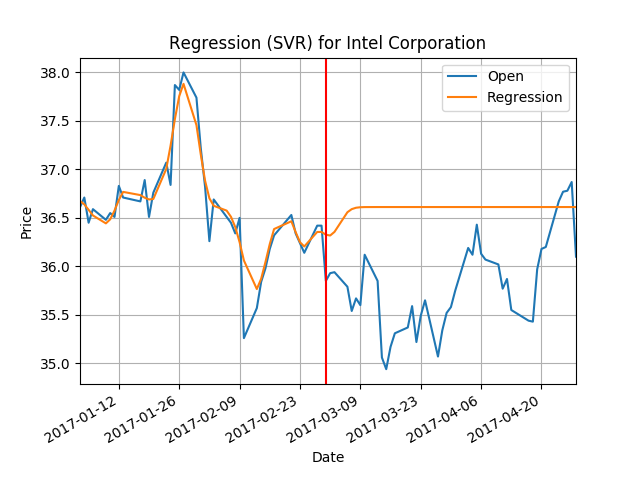
\includegraphics[width=150mm]{pictures/plots/intel_svr_50.png}
\caption{Wykres regresji wektorów nośnych dla 50\% danych uczących, Intel}
\label{fig:intel_svr_50}
\end{figure}

Wykres na rysunku \ref{fig:intel_svr_50} wykazuje poprawne dopasowanie modelu regresji w części danych uczących, lecz w części danych testowych błędnie identyfikuje trend, a krzywa regresji przybiera postać prostej.
Może to być spowodowane błędnym dobraniem parametrów obiektu \textit{SVR()}.\\

\begin{figure}[h!]
\centering
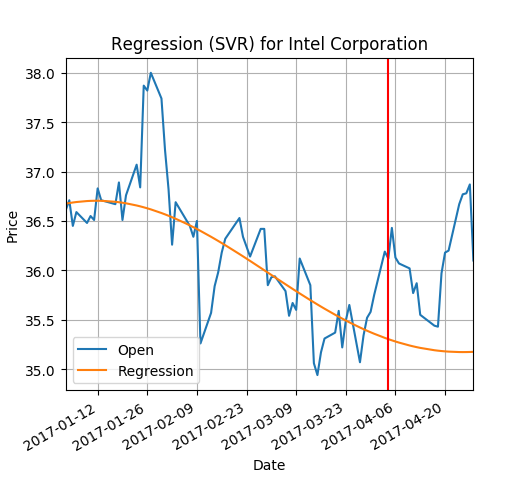
\includegraphics[width=150mm]{pictures/plots/intel_svr_80.png}
\caption{Wykres regresji wektorów nośnych dla 80\% danych uczących, Intel}
\label{fig:intel_svr_80}
\end{figure}

Podobnie jak w przypadku wykresu \ref{fig:intel_krr_80} regresji grzbietowej, także i w powyższym przypadku dopasowanie modelu i identyfikacja trendu spadkowego są zauważalne.\\

\subsection{Regresja Procesu Gaussa}

Na rysunkach \ref{fig:intel_gpr_20}, \ref{fig:intel_gpr_50} i \ref{fig:intel_gpr_80} przedstawiono wykresy analizy regresji procesu Gaussa dla następujących ilośći danych testowych: 20\%, 50\% i 80\%.\\

\begin{figure}[h!]
\centering
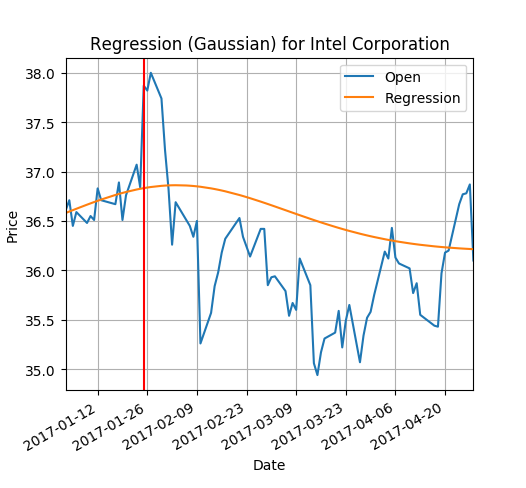
\includegraphics[width=150mm]{pictures/plots/intel_gpr_20.png}
\caption{Wykres regresji procesu Gaussa dla 20\% danych uczących, Intel}
\label{fig:intel_gpr_20}
\end{figure}

W powyższym przypadku krzywa regresji poprawnie identyfikuje trend spadkowy w części testowej, jednakże niewielkie nachylenie krzywej nie oddaje do końca charakteru spadkowego danych.\\ 

\begin{figure}[h!]
\centering
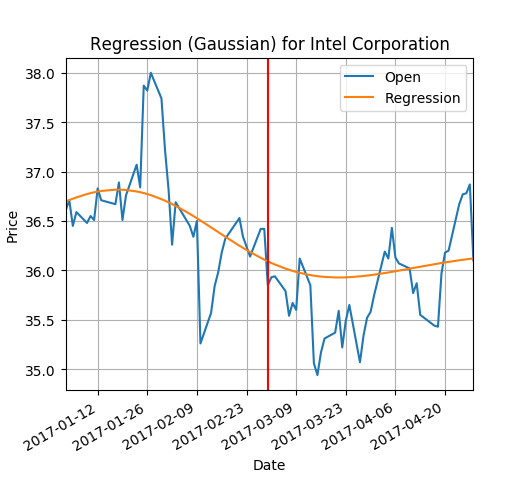
\includegraphics[width=150mm]{pictures/plots/intel_gpr_50.png}
\caption{Wykres regresji procesu Gaussa dla 50\% danych uczących, Intel}
\label{fig:intel_gpr_50}
\end{figure}

Na rysunku \ref{fig:intel_gpr_50} można zaobserwować krzywą regresji poprawnie opisującą i przewidującą przebieg trendu.
W części danych testowych zauważalny jest nie tylko delikatny spadek, lecz również wzrost dla końcowych wartości danych, co zgadza się z wartościami testowymi.\\

\begin{figure}[h!]
\centering
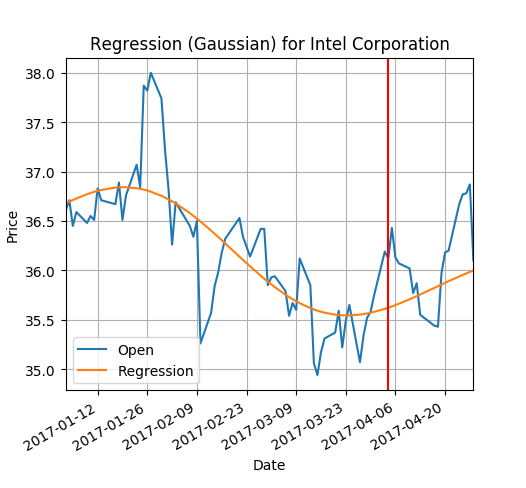
\includegraphics[width=150mm]{pictures/plots/intel_gpr_80.png}
\caption{Wykres regresji procesu Gaussa dla 80\% danych uczących, Intel}
\label{fig:intel_gpr_80}
\end{figure}

W porównaniu do poprzednich wyników regresji procesu Gaussa, powyższy wykres potwierdza wniosek, iż wraz ze wzrostem ilości danych testowych dla tego zbioru danych, rośnie dopasowanie modelu oraz jakość predykcji.\\

\subsection{Podsumowanie}

Dane dotyczące średniego błędu kwadratowego oraz wyników predykcji modeli regresji są przedstawione na wykresach \ref{fig:intel_mean_square} oraz \ref{fig:intel_score}.\\

\begin{figure}[h!]
\centering
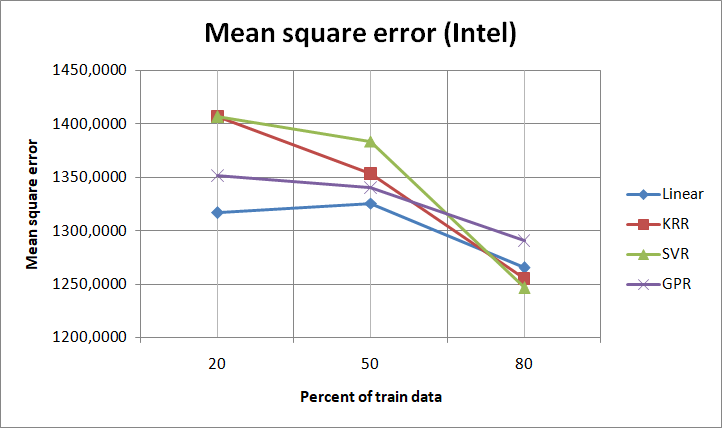
\includegraphics[width=150mm]{pictures/plots/intel_mean_square.png}
\caption{Wykres zmian wartości średniego błędu kwadratowego, Intel}
\label{fig:intel_mean_square}
\end{figure}

\begin{figure}[h!]
\centering
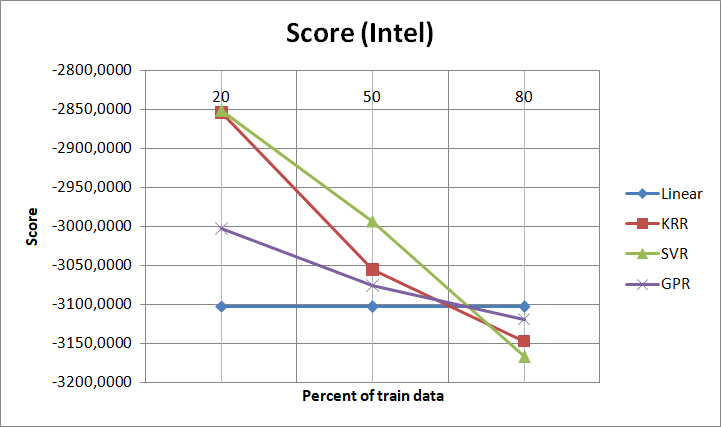
\includegraphics[width=150mm]{pictures/plots/intel_score.png}
\caption{Wykres zmian wartości wyników dopasowania modelu, Intel}
\label{fig:intel_score}
\end{figure}

Z powyższych danych wynika, iż dla ilości danych uczących wynoszącej 20\% najwyższy średni błąd kwadratowy uzyskały modele regresji wektorów nośnych oraz grzbietowa, najniższy zaś model regresji liniowej.
Dla ilości danych uczących wynoszącej 50\% najwyższa wartość błędu odnosi się do modelu regresji wektorów nośnych, a najniższa do modelu regresji liniowej.
Dla 80\% danych uczących natomiast, wszystkie modele regresji osiągnęły podobną, niską wartość, z wyjątkiem modelu regresji procesu Gaussa, który osiągnął wartość najwyższą.\\

W odróżnieniu od poprzedniego testowanego zakresu danych, w tym przypadku zaobserwować można tendencję spadku wartości średniego kwadratu błędów wraz ze wzrostem procentowej ilości użytych danych uczących.\\

Z wykresu \ref{fig:intel_score} wynika, iż wraz ze wzrostem ilości użytych danych uczących spada wartość dopasowania każdego modelu, z wyjątkiem modelu liniowego, który przedstawia za każdym razem podobną wartość.
Może być to spowodowane faktem, iż wartość ta jest liczona jedynie dla danych testowych, więc przy zmniejszaniu ich ilości obserwujemy spadek dopasowania.\\

Analiza wykresów pozwala wnioskować, iż trafne określenie trendu można dostrzec na wykresach regresji procesu Gaussa, liniowej, grzbietowej (80\% danych uczących) oraz wektorów nośnych (80\% danych uczących).
Natomiast niedokładna predykcja trendu widoczna jest na wykresach regresji grzbietowej (20\% i 50\% danych uczących) oraz wektorów nośnych (20\% i 50\% danych uczących).\\

\section{Wnioski}

\begin{enumerate}
 \item Dokładność predykcji modelu regresji liniowej zmienia się nieznacznie w zależności od zmiany proporcji ilości danych uczących względem danych testowych.
 \item Przedstawione modele regresji nieliniowych wykazują dużą wrażliwość na wysoką zmienność danych poddawanych analizie, przez co w celu osiągnięcia bardziej dokłądnych wyników predycji niezbędne jest znalezienie właściwych zakresów parametrów podawanych jako argumenty do obiektów tych regresji.
 \item Wartości średniego kwadratu błędów oraz wyników predykcji (dopasowania modelu) wykazują zależność od całkowitej ilości analizowanych danych. Wraz ze wzrostem ich ilości zwiększają się wartości błędów, a wyniki predykcji ulegają polepszeniu.
 \item Dobre właściwości określania trendu dla obydwu testowanych zakresów danych wykazały: regresja liniowa, wektorów nośnych (przy 80\% danych uczących) oraz grzbietowa (przy 80\% danych uczących).
 \item Regresja procesu Gaussa w przypadku dużego zbioru danych nie wykazała dobrych zdolności predykcyjnych, natomiast w przypadku małego zbioru można ją uznać za najlepszą metodę regresji dla podanych warunków.
 \item Jakość predykcji za pomocą testowanych metod w dużym stopniu zależy od struktury danych użytych do analizy. Jednocześnie najbardziej odporną na ten czynnik metodą okazała się regresja liniowa.
 \item Wraz ze wzrostem ilości użytych do analizy danych uczących, w większości przypadków wzrasta trafność predykcji lub trafność określenia trendu.
 \item Pakiet \textit{Scikit-learn} i udostępniane przez niego metody regresji są przydatne w analizie danych giełdowych. Ich dokładność można zwiększyć odpowiednio parametryzując tworzone obiekty modeli regresji, oraz poprawnie dobierając dane.
\end{enumerate}

